\documentclass[11pt,]{article}
\usepackage{lmodern}
\usepackage{amssymb,amsmath}
\usepackage{ifxetex,ifluatex}
\usepackage{fixltx2e} % provides \textsubscript
\ifnum 0\ifxetex 1\fi\ifluatex 1\fi=0 % if pdftex
  \usepackage[T1]{fontenc}
  \usepackage[utf8]{inputenc}
\else % if luatex or xelatex
  \ifxetex
    \usepackage{mathspec}
    \usepackage{xltxtra,xunicode}
  \else
    \usepackage{fontspec}
  \fi
  \defaultfontfeatures{Mapping=tex-text,Scale=MatchLowercase}
  \newcommand{\euro}{€}
\fi
% use upquote if available, for straight quotes in verbatim environments
\IfFileExists{upquote.sty}{\usepackage{upquote}}{}
% use microtype if available
\IfFileExists{microtype.sty}{%
\usepackage{microtype}
\UseMicrotypeSet[protrusion]{basicmath} % disable protrusion for tt fonts
}{}
\usepackage[margin=1.0in]{geometry}
\ifxetex
  \usepackage[setpagesize=false, % page size defined by xetex
              unicode=false, % unicode breaks when used with xetex
              xetex]{hyperref}
\else
  \usepackage[unicode=true]{hyperref}
\fi
\hypersetup{breaklinks=true,
            bookmarks=true,
            pdfauthor={},
            pdftitle={Preprinting Microbiology},
            colorlinks=true,
            citecolor=blue,
            urlcolor=blue,
            linkcolor=magenta,
            pdfborder={0 0 0}}
\urlstyle{same}  % don't use monospace font for urls
\usepackage{graphicx,grffile}
\makeatletter
\def\maxwidth{\ifdim\Gin@nat@width>\linewidth\linewidth\else\Gin@nat@width\fi}
\def\maxheight{\ifdim\Gin@nat@height>\textheight\textheight\else\Gin@nat@height\fi}
\makeatother
% Scale images if necessary, so that they will not overflow the page
% margins by default, and it is still possible to overwrite the defaults
% using explicit options in \includegraphics[width, height, ...]{}
\setkeys{Gin}{width=\maxwidth,height=\maxheight,keepaspectratio}
\setlength{\parindent}{0pt}
\setlength{\parskip}{6pt plus 2pt minus 1pt}
\setlength{\emergencystretch}{3em}  % prevent overfull lines
\providecommand{\tightlist}{%
  \setlength{\itemsep}{0pt}\setlength{\parskip}{0pt}}
\setcounter{secnumdepth}{0}

%%% Use protect on footnotes to avoid problems with footnotes in titles
\let\rmarkdownfootnote\footnote%
\def\footnote{\protect\rmarkdownfootnote}

%%% Change title format to be more compact
\usepackage{titling}

% Create subtitle command for use in maketitle
\newcommand{\subtitle}[1]{
  \posttitle{
    \begin{center}\large#1\end{center}
    }
}

\setlength{\droptitle}{-2em}
  \title{\textbf{Preprinting Microbiology}}
  \pretitle{\vspace{\droptitle}\centering\huge}
  \posttitle{\par}
  \author{}
  \preauthor{}\postauthor{}
  \date{}
  \predate{}\postdate{}

% Redefines (sub)paragraphs to behave more like sections
\ifx\paragraph\undefined\else
\let\oldparagraph\paragraph
\renewcommand{\paragraph}[1]{\oldparagraph{#1}\mbox{}}
\fi
\ifx\subparagraph\undefined\else
\let\oldsubparagraph\subparagraph
\renewcommand{\subparagraph}[1]{\oldsubparagraph{#1}\mbox{}}
\fi

\usepackage{helvet} % Helvetica font
\renewcommand*\familydefault{\sfdefault} % Use the sans serif version of the font
\usepackage[T1]{fontenc}

\usepackage[none]{hyphenat}

\usepackage{setspace}
\doublespacing
\setlength{\parskip}{1em}

\usepackage{lineno}

\usepackage{pdfpages}
\usepackage{comment}

\begin{document}
\maketitle

\begin{center}
\vspace{25mm}
Patrick D. Schloss${^\dagger}$

\vspace{30mm}

$\dagger$ To whom correspondence should be addressed: pschloss@umich.edu; Department of Microbiology and Immunology, University of Michigan, Ann Arbor, MI

\vspace{10mm}

\textbf{Format:} Perspective or Commentary

\textbf{Number of words:} \textasciitilde4500 plus references, figures, and abstract

\end{center}

\newpage

\linenumbers

\subsection{Abstract}\label{abstract}

The field of microbiology has experienced significant growth due to
transformative advances in technology and the influx of scientists
driven by a curiosity to understand how bacteria, archaea, microbial
eukaryotes, and viruses interact with each other and their environment
to sustain myriad biochemical processes that are essential for
maintaining the Earth. With this explosion in scientific output, a
significant bottleneck has been the ability to disseminate this new
knowledge to peers and the public in a timely manner. Preprints have
emerged as a tool that a growing number of microbiologists are using to
overcome this bottleneck and to recruit in an effective and transparent
way a broader pool of reviewers prior to submitting to traditional
journals. Although use of preprints is still limited in the biological
sciences, early indications are that preprints are a robust tool that
can complement and enhance peer-reviewed publications. As publishing
moves to embrace advances in internet technology, there are many
opportunities for preprints and peer-reviewed journals to coexist in the
same ecosystem.

\newpage

\textbf{\emph{Background.}} Many scientists, including microbiologists,
have begun to use preprints and other online venues such as social
media, blog posts, and videos as methods to garner attention for their
research and to engage the public. A preprint is an interim research
product, such as an unpublished manuscript, made publicly available
before going through an official peer-review process (1--4). Authors can
post their manuscript to a preprint server for others to read, share,
and comment. Preprints were initially adopted among physicists and
biologists in the 1960s as a method of sharing interesting research
amongst colleagues (5). While the biological community's commitment to
preprints waned, the physics community adopted what is now the
\emph{arXiv} (pronounced ``archive'') preprint server that was hosted at
the Los Alamos National Laboratories from 1991 to 1999 and then at
Cornell University (6). For some physicists and mathematicians, posting
a preprint to \emph{arXiv} followed by submission to a peer-reviewed
journal has become a standard publication pathway. Although \emph{arXiv}
has hosted a number of computational biology papers, the server has not
drawn widespread attention from biologists. Among proponents of
\emph{arXiv}, preprints have aided in the development of research
communication by accelerating the release of the science and helping it
to achieve a wider audience for critique and reception (7). Considering
the broadening adoption of preprints among microbiologists, I sought to
explore the specific uses of and concerns regarding preprints.

\textbf{\emph{Landscape of preprint servers.}} In 2013, two preprint
servers, the \emph{bioRxiv} (pronounced ``bio-archive'') and \emph{PeerJ
Preprints}, were launched as preprint servers for biologists that would
parallel \emph{arXiv} (8). Both platforms offer similar features:
preprint posting is free; each preprint receives a digital object
identifier (DOI) that facilitates the ability to cite preprints in other
scholarly work; if the preprint is ever published, the preprint is
linked to the published version; the submission process for both options
is relatively simple allowing authors to upload a PDF version of their
preprint and supplemental materials; preprints are typically publicly
available in about 24 hours; they have built in venues for authors to
discuss their research with people who leave comments on the manuscript;
preprints undergo a basic screening process to remove submissions with
offensive or non-scientific content; and the sites provide article-level
metrics indicating the number of times an abstract has been accessed or
the preprint has been downloaded. There are several important
differences between the two options. First, \emph{PeerJ Prints} is a
for-profit organization and \emph{bioRxiv} is a non-profit organization
sponsored by Cold Spring Harbor Laboratory. This difference can be
meaningful to authors since some journals, including the American
Society for Microbiology (ASM) Journals, will only accept submissions
that have been posted on preprint servers hosted by non-profit
organizations. Second, preprints at \emph{PeerJ Preprints} are posted
under the Creative Commons Attribution License (CC-BY) and
\emph{bioRxiv} preprints can be posted under one of four CC-BY licenses
or with no permission for reuse. This can be relevant for authors hoping
to submit their work to a journal as journals will not consider
manuscripts posted as preprints under a CC-BY license (e.g.
\emph{Proceedings of the National Academy of Sciences}). The flexibility
of the \emph{bioRxiv} licensing empowers authors to choose the model
that best suits them, while ensuring the rapid posting of their research
results however, it is important to provide clear information to authors
on the legal and practical tradeoffs of each option. A cosmetic, but
still relevant difference between the two is the layout and feel of the
two websites. Compared to the \emph{bioRxiv} site, the \emph{PeerJ
Preprint} site is more fluid, gives readers the ability to ``follow'' a
preprint, and provides better access to article keywords and the ability
to search preprints. With broader acceptance of preprints by traditional
journals, many journals, including all of the ASM journals, have
established mechanisms to directly submit manuscripts that are posted as
preprints on \emph{bioRxiv}. It is only possible to transfer a
\emph{PeerJ Preprint} for submission to \emph{PeerJ}. In many ways,
preprint servers have taken on the feel of a journal. As adoption of
this approach expands, it is likely that the features of these sites
will continue to improve. It is also likely that interfaces from
third-parties will improve. For example, although Google Scholar
includes preprints hosted at \emph{bioRxiv} and \emph{PeerJ Preprints}
in their search results, PubMed and Web of Science do not. There is also
hope that the National Institutes of Health (NIH) will renew their
interest in indexing preprints as separate research products than
peer-reviewed publications. As preprint servers begin to look and act
like traditional journals by incorporating features and interfaces, it
is important to value the strength of the preprint - that of an interim
research product, nimble and quickly posted. It is therefore essential
to balance the requirements placed on authors for features associated
with preprints with the current desirable efficiency of the preprint
format.

\textbf{\emph{Specific challenges for microbiology.}} Although preprints
offer an efficient and novel venue for disseminating microbiology
research, there are several considerations that the scientific community
and those that oversee preprint servers must consider. It is critical
that assurances be given that policies are in place to address these
issues. First, a significant amount of attention has to be given to the
potential dual use research of concern (DURC) since posted results in
microbiology research could offer insights to individuals seeking to
engage in terrorist activities. Second, for researchers engaging in
research that involves human subjects it is critical that assurances be
made that institutional review boards have been consulted and have
approved of the research. Third, there is significant concern regarding
researchers hiding potential conflicts of interest that could affect a
project's experimental design, analysis, and interpretation of results.
Finally, recent expansions in scientific publishing have revealed
numerous cases of plagiarism or misconduct. Again, while hoping to
maintain the efficiency of the preprint format, traditional microbiology
journals have policies for these issues in place that should be easy to
implement by preprint servers.

\textbf{\emph{Acceptance of preprints by journals.}} An early
controversy encountered by researchers interested in posting their work
as preprints as a stage in disseminating their research was whether it
constituted prior publication. The broad consensus at this point is that
preprints do not constitute prior publication. This consensus is
reflected in the current policies of journals that commonly publish
microbiology research including those published by ASM, the Microbiology
Society, International Society for Microbial Ecology, PLOS, the
\emph{Proceedings of the National Academy of Science}, \emph{Science},
\emph{Nature} and Cell press, which each take a generally permissive
stance towards prior posting of preprints prior to submission.
Considering the relatively fluid nature of many of these policies and
the journals' specific policies, prospective authors should be aware of
the positions taken by the journals where they may eventually submit
their work. Comprehensive lists of journals' attitudes towards preprints
are available online and are regularly updated (9, 10).

\textbf{\emph{Preprints and peer-review.}} The use of preprints for
citations in other scientific reports and grant proposals has been
called into question because preprints upend the traditional peer-review
editorial process (11). It is important to note that the peer-review
process was adapted to the technologies and trends that have evolved
over the past 100 years. The formal peer-review system that most
journals currently use was not developed until the end of the 1800s with
the advent of typewriters and carbon paper (12). Editorial decisions
were typically made by a single person or a committee (i.e.~the
editorial board) who had an expertise that covered the scope of the
journal. As science became more specialized, new journals would form to
support and provide a source of validation to the new specialty. The
growth in science in the mid 1900s resulted in a shift from journals
struggling to find sufficient numbers of manuscript to publish to having
too many manuscripts submitted. It has been argued that the widespread
adoption of decentralized peer-review was due to the increased
specialization and to deal with the large number of manuscript
submissions (13). Peer-review did not achieve widespread use at many
journals, including the \emph{Journal of Bacteriology}, until the 1940s
and 1950s. Thus the ``tradition'' of peer-review is only 70 years old.
Given the rapid advances in communication technology and even greater
specialization within microbiology, it is worth pondering whether the
current scientific publishing system and peer-review system, in
particular, need to continue to adapt with our science.

Communicating research has traditionally been done within research group
meetings, departmental seminars, conferences, and as publications. Along
this continuum, there is an assumption that the quality of the science
has been improved because it has been vetted by more experts in the
field. The public dissemination of one's research is a critical
component of the scientific method. By describing their research,
scientists subject their work to formal and informal peer review. Their
research is scrutinized, praised, and probed to identify questions that
help seed the next iteration of the scientific method. A common critique
of more modern approaches to publishing has been an inability to assess
the quality of the science without the validation of peer-review.
Attached to assertions of the validity of the research has been
assertions of the impact and robustness of the research. These are all
quality assessments that many acknowledge are difficult to assess by the
traditional peer-review process. This has led to some journals, most
notably \emph{PLOS ONE}, calling for referees to place a reduced
emphasis on the perceived impact or significance of the work. It has
also led to the call for replacing or complementing pre-publication
peer-review with post-publication peer-review using PubMed Commons,
PubPeer, journal-based discussion forums, F1000Research, and other
mechanisms. Alas if scientists are going to depend on post-publication
peer-review or informal methods of peer-review for documents like
preprints, they must be willing to provide constructive feedback on the
work of others.

\textbf{\emph{Preprints have the potential to change the advancement of
science.}} Preprints are often viewed as existing in a state of
scientific limbo. As noted above, they represent a formal communication,
but an interim one, not officially published. As the use of preprints
grows and scientists' perceptions of preprints matures, there are a
number of issues that will need to be addressed.

First, a common concern is that if a researcher posts their work as a
preprint, it will be ``scooped'' by another researcher and the preprint
author will lose their ability to claim primacy or their ability to
publish the work in a journal. Considering the preprint is a citable
work with a DOI, it would, in fact, be the preprint author that scooped
the second. The use of preprints uncouples the communication of the
discovery from the relevance of the discovery, which will come later
based on peer-review, comments from other scientists at meetings or
online, and eventually citations. A growing number of scientific
societies and journals, including ASM view preprints as citable and as
having a legitimate claim to primacy (1, 14--16). Some scientists worry
that with such protection a researcher can make a claim without valid
data to support their claims (3). This is possible; however, it is also
the responsibility of the scientific community to utilize the
peer-review mechanisms that are available to comment on those preprints
pointing out methodological problems or to indicate that they are
speaking beyond the data.

A second area of concern is whether a preprint can be used to support a
grant proposal. Given the length limitations placed on grant proposals
by funding agencies, there is a push to cite previous work to indicate a
research team's competence in an area or to provide preliminary data.
Some fear that the use of preprints will allow scientists to circumvent
page limits by posting preliminary manuscripts. I would hope that both
consumers of preprints and grant proposal reviewers would be able to
differentiate between someone trying to game the system and someone that
is using preprints as a mechanism to improve their science. This would
be greatly facilitated if funding agencies would include preprints as
evidence for research progress, but listed separately from peer-reviewed
publications to help review panels in their decisions and to help author
substantiate evidence they feel they need to provide.

A third concern is what role preprints should have in assessing a
scientist's productivity. Clearly use of publication metrics as an
indicator of a scientist's productivity and impact is a contentious
topic without even discussing the role of preprints. Regardless, given
the propensity for researchers to list manuscripts as being ``in
preparation'' or ``in review'' on an application or curriculum vitae,
listing them instead as preprints that can be reviewed by a committee
would significantly enhance an application and a reviewer's ability to
judge the application. In fact, several funding agencies including the
Wellcome Trust and the UK Medical Research Council encouraging
fellowship applicants to include preprints in their materials;
meanwhile, the NIH is in the process of soliciting input from the
scientific community on their role in grant applications. Others are
mandating that researchers post preprints for all of their work prior to
submitting the work to a journal (17).

Beyond these concerns, preprints are also causing some to change their
publication goals. Some authors are explicitly stating that a preprint
will not be submitted to a journal (18). Although these authors may be a
minority of those who post preprints, such an approach may be attractive
to those who need to cite a report of a brief research communication, a
critique of another publication, or negative results. It is clear that
the adoption of preprints will challenge how scientists interact and
evaluate each other's work. There is great potential to empower
researchers by controlling when a citable piece of work is made public.

\textbf{\emph{Microbiology anecdotes.}} The peer-review editorial
process can be lengthy and adversarial. In contrast, preprints represent
a rapid and potentially collaborative method for disseminating research.
Several anecdotes from the microbiology literature are emblematic of
benefits of the rapid release cycle that is inherent in the use of
preprints.

First, preprints have proven useful for rapidly disseminating results
for disease outbreaks and new technologies. Prior to the recent Zika
virus outbreak there were approximately 50 publications that touched on
the biology and epidemiology of the virus; as of January 2017 the number
of Zika virus-related publications was over 1,700. During the recent
outbreak, more than 110 Zika virus-related preprints have been posted at
\emph{bioRxiv}. Any manuscript that was published went through several
month delays in releasing information to health care workers, the
public, and scientists needing to learn new methods to study a
previously obscure virus. In contrast, those that posted their work as a
preprint were able to disseminate their methods and results instantly.
Over the last several years there have also been rapid advances in DNA
sequencing technologies have fundamentally changed how microbial science
is performed. One notable technology, the MinIon sequencing platform
from Oxford Nanopore, has received considerable attention from
researchers who have posted more than 90 preprints describing new
MinIon-based methods and results to preprint servers. For such a rapidly
developing technology, the ability to share and consume methods from
other scientists has created a feed forward effect where the technology
has likely advanced at a faster rate than it otherwise would have.

Second, preprints have proven useful for rapidly correcting the
scientific literature. On February 9, 2015, \emph{Cell Systems} posted a
study by Afshinnekoo et al. online (19). The study collected and
analyzed metagenomic sequence data from the New York City subway system
and reported finding \emph{Yersinia pestis} and \emph{Bacillus
anthracis}. Because of the focus on these two bioterrorism agents, this
study generated a considerable amount of media attention. On April 25,
2015, Petit et al. (20) posted a preprint to Zenodo demonstrating that
there was no evidence for \emph{B. anthracis} in the dataset. On July
29, 2015, a critique was published by \emph{Cell Systems} along with a
response from the original authors offering a correction to their
manuscript (21, 22). A second anecdote of using preprints to aid in
post-publication peer-review surrounds the publishing of a draft
tardigrade genome in \emph{The Proceedings of the National Academy of
Sciences}. On November 23, 2015 a study by Boothby et al. (23) was first
published online. The authors claimed that 17.5\% of its genes came from
bacteria, archaea, fungi, plants, and viruses. Another group had been
analyzing sequence data from a parallel tardigrade genome sequencing
project and did not observe the same result. A week later, on December
1, 2015, the second group had posted a preprint comparing the two genome
sequences and demonstrating that the exciting claims of horizontal gene
transfer were really the product of contaminants (24); this analysis
would eventually be published online by the original journal on March
24, 2016 followed by a rebuttal by the original authors on May 31, 2016
(25, 26). Two other analyses of the original data were published in May
2016 and a third was posted as a preprint on February 2, 2016 (27--29).
These anecdotes underscore the value of having a rapid posting cycle to
correcting errors in the scientific literature and that results posted
to preprint servers were able to correct the record within weeks of the
initial publication while the traditional path took six months in both
cases. A final notable case where preprints have accelerated the
correction of the scientific record was a preprint posted by Bik et al.
reporting numerous cases of image manipulation in peer reviewed studies
(30). Their preprint was posted on April 20, 2016 and published in
\emph{mBio} on June 7, 2016 (31). Instead of using preprints to react to
published papers that have been through peer review, it would be
interesting to consider how the editorial process for these examples and
the infamous ``Arsenic Life'' paper (32) would have been different had
they initially been posted as preprints.

\textbf{\emph{Metrics for microbiology-affiliated preprints.}} To
analyze the use of preprints, I downloaded the \emph{bioRxiv} on
December 31, 2016. I chose to analyze \emph{bioRxiv} preprints because
these preprints are amenable for submission to ASM journals and there
were 7,434 \emph{bioRxiv} preprints compared to the 2,650 available at
\emph{PeerJ Preprint}. Among the 7,434 preprints on bioRxiv, 329 were
assigned by the authors into the Microbiology category. One limitation
of the \emph{bioRxiv} interface is the inability to assign manuscripts
to multiple categories or to tag the content of the preprint. For
example, this manuscript could be assigned to either the Microbiology or
the Scientific Communication and Education categories. To counter this
limitation, I developed a more permissive approach that classified
preprints as being microbiology-affiliated if their title or abstract
had words containing \emph{yeast}, \emph{fung}, \emph{viral},
\emph{virus}, \emph{archaea}, \emph{bacteri}, \emph{microb},
\emph{microorganism}, or \emph{pathogen}. I identified 1,228 additional
manuscripts that I considered microbiology-affiliated. These
microbiology-affiliated preprints were primarily assigned to the
Evolutionary Biology (N=221), Genomics (N=184), or Bioinformatics
(N=182) categories.

As the total number of preprints has grown exponentially since the
creation of \emph{bioRxiv}, submission of microbiology-affiliated
preprints has largely followed this growth (\textbf{Figure 1A}).
Although preprints are still relatively new, the collection of
microbiology-affiliated preprints indicates widespread experimentation
with the format and considerable geographic diversity. Reflecting the
still relatively novelty of preprints, 1,132 (86.1\%) corresponding
authors who submitted a microbiology-affiliated preprint (N=1,314 total)
have posted a single preprint and 3.6\% have posted 3 or more preprints.
Corresponding authors that have posted microbiology-affiliated preprints
are from 60 countries and are primarily affiliated with institutions in
the United States (50.8\% of microbiology-affiliated preprints), United
Kingdom (11.9\%), and Germany (4.2\%). As the preprint format matures,
it will be interesting to see whether the fraction of authors that post
multiple preprints increases and whether the geographic diversity
amongst those authors is maintained.

As stated above, preprints offer researchers the opportunity to improve
the quality of their work by adding a more formal and public step to the
scientific process. Among the microbiology-affiliated preprints, 146
(9.3\%) had been commented on at least once and only 35 (2.2\%) more
than three times using the \emph{bioRxiv}-hosted commenting feature.
Although the hosted commenting is only one mechanism for peer review,
this result was somewhat disturbing since the preprint model implicitly
depends on people's willingness to offer others feedback. Although it is
not in the tradition of the scientific community to comment publicly
online about colleagues' research results, I am optimistic that this
will change given the possibilities of new media, and possibly
incentives for open commenting and reviewing could shift the trend.
Importantly, authors do appear to be incorporating feedback from
colleagues or editorial insights from journals as 404 (25.8\%) of
preprints were revised at least once. Among the preprints posted prior
to January 1, 2016, 31.6\% of the Microbiology category preprints,
35.1\% of the microbiology-affiliated preprints, and 33.8\% of all
preprints have been published. As noted above, not all authors submit
their preprints to journals. This would indicate that the ``acceptance
rates'' are actually higher. Regardless, considering that these
acceptance rates are higher than many peer-reviewed journals
(e.g.~approximately 20\% at ASM Journals), these results dispel the
critique that preprints represent overly preliminary research.

Measuring the impact and significance of scientific research is
notoriously difficult. Using several metrics I sought to quantify the
effect that broadly defined microbiology-affiliated preprints have had
on the work of others. Using the download statistics associated with
each preprint, I found that the median number of times an abstract or
PDF had been accessed was 923 (IQR: 603 to 1445) and 303 (IQR: 167 to
568), respectively. These values represent two aspects of posting a
preprint. First, they reflect the number of times people were able to
access science before it was published. Second, they reflect the number
of times people were able to access a version of a manuscript that is
published behind a paywall. To obtain a measure of a preprint's ability
to garner attention and engage the public, I obtained the Altmetric
Attention Score for each preprint (\textbf{Figure 1B}). The Altmetric
Attention Score measures the number of times a preprint or paper is
mentioned in social media, traditional media, Wikipedia, policy
documents, and other sources (33). A higher score indicates that a
preprint received more attention. Microbiology-affiliated preprints have
had a median Altmetric Attention Score of 7.3 (IQR: 3.2 to 16.3) and
those of all preprints hosted at \emph{bioRxiv} have had a median score
of 7.0 (IQR: 3 to 15.6). For comparison, the median Altmetric Attention
Score for articles published in \emph{mBio} published since 2013 was 4.5
(IQR: 1.2 to 13.6). Of all scholarship tracked by Altmetric, the median
Altmetric Attention Score for preprints posted at \emph{bioRxiv} ranks
at the 86 percentile (IQR: 66 to 94. A more traditional and
controversial metric of impact has been the number of citations an
article receives. I obtained the number of citations for the published
versions of manuscripts that were initially posted as preprints. To
allow for a comparison to traditional journals, I considered the
citations for preprints published in 2014 and 2015 as aggregated by Web
of Science (\textbf{Figure 1C}). Among the preprints that were published
and could be found in the Web of Science database, the median number of
citations was 6.5 (IQR: 2-14; mean: 13.6). For comparison, for the
papers published in \emph{mBio} in 2014 and 2015, the median number of
citations was 5 (IQR: 2-9; mean: 6.7). Although it is impossible to
quantify the quality or impact of research with individual metrics, it
is clear that preprints and the publications that result from them are
broadly accepted by the microbiology community.

\textbf{\emph{Preprints from an author's perspective.}} Posting research
as a preprint gives an author great control over when their work is made
public. Under the traditional peer-review model, an author may need to
submit and revise their work multiple times to several journals over a
long period before it is finally published. In contrast, an author can
post the preprint at the start of the process for others to consume and
comment on as it works its way through the editorial process. A first
example illustrates the utility of preprints for improving access to
research and the quality of its reporting. In 2014, my research group
posted a preprint to \emph{PeerJ Preprints} describing a method of
sequencing 16S rRNA gene sequences using the Pacific Biosciences
sequencing platform (34). At the same time, they submitted the
manuscript for review at \emph{PeerJ}. While the manuscript was under
review, they received feedback from an academic scientist and from
scientists at Pacific Biosciences that the impact of the results could
be enhanced by using a recently released version of the sequencing
chemistry. Instead of ignoring this feedback and resubmitting the
manuscript to address the reviews, we generated new data and submitted
an updated preprint a year later with a simultaneous submission to
\emph{PeerJ} that incorporated the original reviews as well as the
feedback we received from the academic scientist and Pacific
Biosciences. It was eventually published by \emph{PeerJ} (35, 36). Since
2015, we have continued to post manuscripts as preprints at the same
time as we have submitted manuscripts. Although the feedback to other
manuscripts has not been as helpful as our initial experience, we were
able to sidestep lengthy review processes by immediately making our
results available; in one case our preprint was available 7 months ahead
of the final published version (37, 38). As a second example, this
manuscript was posted to \emph{bioRxiv} as a preprint on
\textbf{February XX, 2017}. I then solicited feedback on the manuscript
using social media. Two weeks later, I incorporated the comments and
posted a revised preprint and submitted the manuscript to \emph{mBio}.
During that time, the abstract was read \textbf{XXXX} times and the PDF
was accessed \textbf{XXXX} times. This process engaged \textbf{XXXX}
commenters on \emph{bioRxiv}, \textbf{XXXX} people on Twitter,
\textbf{XXXX} on Facebook, and \textbf{XXXX} via email. I received
useful feedback from \textbf{XXX} people. Compared to the two or three
scientists that typically review a manuscript, this experience engaged a
much larger and more diverse community than had I foregone the posting
of a preprint. Although there are concerns regarding the quality of the
science posted to a preprint server, I contend that responsible use of
preprints as a part of the scientific process can significantly enhance
the science.

\textbf{\emph{Preprints from a publisher's perspective.}} A lingering
question is what role traditional journals will have in disseminating
research if there is broad adoption of preprints. Edited peer-reviewed
journals offer and will continue to offer significant added value to a
publication. A scholarly publishing ecosystem in which preprints coexist
with journals will allow authors to gain value from the immediate
communication of their work associated with preprints and also benefit
from the peer-reviewed, professionally edited publication that
publishers can provide. The professional copyediting, layout, and
publicity that these publishers offer are also unique features of
traditional journals. An alternative perspective is that preprints will
eventually replace traditional journals. Certainly, this is a radical
perspective, but it does serve to motivate publishers to capture the
innovation opportunities offered by preprints. By adopting
preprint-friendly policies, journals can create an attractive
environment for authors. As discussed above, a growing number of
journals have created mechanisms for authors to directly submit
preprints to their journals. An example is offered by the ASM, which
earlier this year launched a new venture from \emph{mSphere}.
mSphereDirect is a publication track of the journal that capitalizes on
the opportunity offered to couple preprints with rigorous peer-review.
mSphereDirect. actively encourages authors to post their manuscripts as
preprints as part of an author-driven editorial process where an
editorial decision is rendered within five days and publication in
\emph{mSphere} within a month (39). ASM is developing a new platform,
MicroNow, which will help coalesce specific communities within the
microbial sciences, further enhancing the use of preprints as well as
published articles (Stefano Bertuzzi, personal communication). In
addition to integrating preprints into the traditional editorial
process, several professional societies have also explicitly supported
citation of preprints in their other publications and recognize the
priority of preprints in the literature (14--16). These are policies
that empower authors and make specific journals more attractive. Other
practices have great potential to improve the reputation of journals. As
measured above, preprints are able to garner attention on par with
papers published in highly selective microbiology journals. Thus, it is
in a journal's best interest to recruit these preprints to their
journals. Several journals including \emph{PLOS Genetics} and
\emph{Genome Biology} have publicly stated that they scout preprints for
this purpose (40, 41). Preprints can also be viewed as a lost
opportunity to journals. A preprint that garners significant attention
may be ignored when it is finally published, brining little additional
attention to the journal. Going forward, it will be interesting to see
the innovative approaches that publishers develop so that they can
benefit by incorporating preprints into their process and whether
publishers' influence is reduced by the widespread adoption of
preprints.

\textbf{\emph{Conclusions.}} An increasing number of microbiologists are
posting their unpublished work to preprint severs as an efficient method
for disseminating their research prior to peer review. A number of
critical concerns remain about how widespread their adoption will be,
how they will be perceived by traditional journals and other scientists,
and whether traditional peer-review will adapt to the new scientific
trends and technologies. Regardless, preprints should offer a great
opportunity for both scientists and journals to publish high quality
science.

\subsection{Acknowledgements}\label{acknowledgements}

I am grateful to Stefano Bertuzzi and Lynn Enquist for their helpful
comments on earlier versions of this manuscript. This work was supported
in part by funding to PDS from the National Institutes of Health
(P30DK034933). I appreciate the support of Altmetric, Inc and Thompson
Reuters who provided advanced programming interface (API) access to
their databases. The workflow utilized commands in GNU make (v.3.81),
GNU bash (v.4.1.2), and R (v.3.3.2). Within R I utilized the cowplot
(v.0.6.9990), dplyr (v.0.5.0), ggplot2 (v.2.1.0.9001), httr (v.1.2.1),
RCurl (v.1.95-4.8), rentrez (v.1.0.4), rjson (v.0.2.15), rvest
(v.0.3.2), sportcolors (v.0.0.1), and tidyr (v.0.6.0) packages. A
reproducible version of this manuscript and analysis is available at
\url{http://www.github.com/SchlossLab/Schloss_PrePrints_mBio_2017}.

\newpage

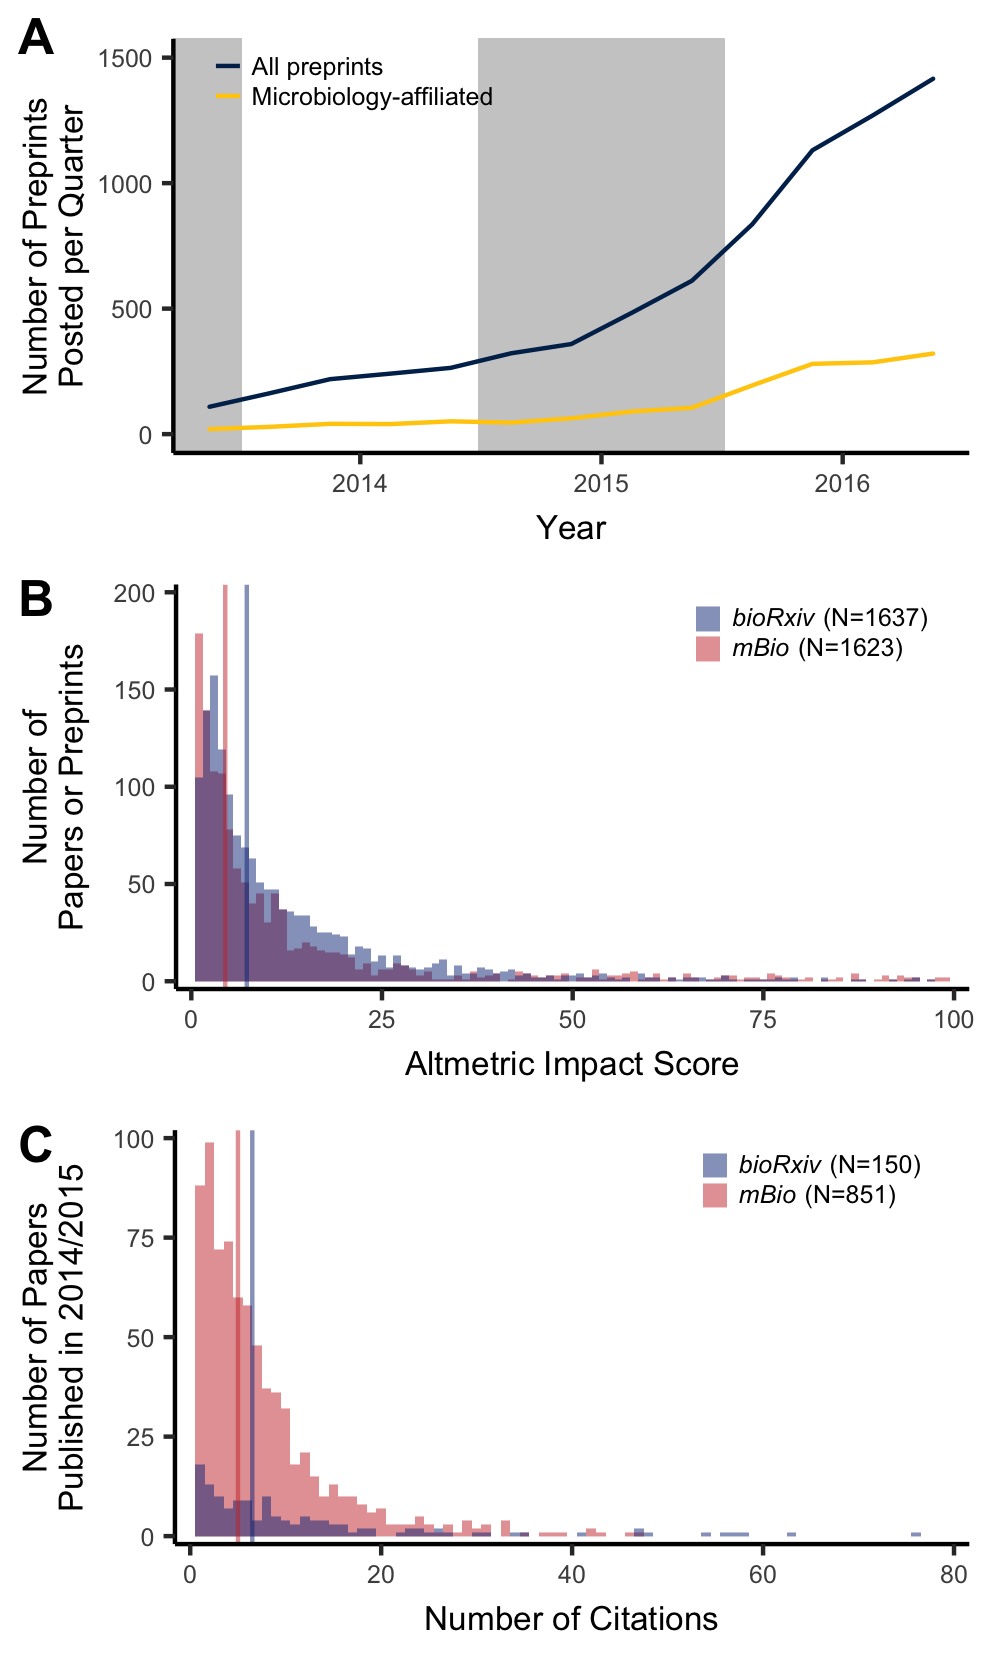
\includegraphics[width=3.5in]{../figures/figure1.png}

\textbf{Figure 1. Summary of microbiology-affiliated preprints since the
creation of} \textbf{\emph{bioRxiv.}} The total number of preprints
posted for each quarter ending December 31, 2016 has largely tracked the
overall submission of preprints to \emph{bioRxiv} (A). The Altmetric
attention scores of preprints posted to \emph{bioRxiv} are similar to
those published in \emph{mBio} since November 2013 indicating preprints
engender a similar level of attention (B). The number of times preprints
that were published in 2014 and 2015 have been cited is similar to the
number of citations for papers published in \emph{mBio} in 2014 and 2015
indicates that published preprints are frequently cited (C). Regions
with common background shading in A are from the same year. The vertical
lines in B and C indicate the median Altmetric impact score and the
median number of citations.

\newpage

\hyperdef{}{references}{\label{references}}
\subsection*{References}\label{references}
\addcontentsline{toc}{subsection}{References}

\hyperdef{}{ref-Vale2015}{\label{ref-Vale2015}}
1. \textbf{Vale RD}. 2015. Accelerating scientific publication in
biology. Proceedings of the National Academy of Sciences
\textbf{112}:13439--13446.
doi:\url{http://doi.org/10.1073/pnas.1511912112}.

\hyperdef{}{ref-DesjardinsProulx2013}{\label{ref-DesjardinsProulx2013}}
2. \textbf{Desjardins-Proulx P}, \textbf{White EP}, \textbf{Adamson JJ},
\textbf{Ram K}, \textbf{Poisot T}, \textbf{Gravel D}. 2013. The case for
open preprints in biology. PLoS Biology \textbf{11}:e1001563.
doi:\url{http://doi.org/10.1371/journal.pbio.1001563}.

\hyperdef{}{ref-Berg2016}{\label{ref-Berg2016}}
3. \textbf{Berg JM}, \textbf{Bhalla N}, \textbf{Bourne PE},
\textbf{Chalfie M}, \textbf{Drubin DG}, \textbf{Fraser JS},
\textbf{Greider CW}, \textbf{Hendricks M}, \textbf{Jones C},
\textbf{Kiley R}, \textbf{King S}, \textbf{Kirschner MW},
\textbf{Krumholz HM}, \textbf{Lehmann R}, \textbf{Leptin M},
\textbf{Pulverer B}, \textbf{Rosenzweig B}, \textbf{Spiro JE},
\textbf{Stebbins M}, \textbf{Strasser C}, \textbf{Swaminathan S},
\textbf{Turner P}, \textbf{Vale RD}, \textbf{VijayRaghavan K},
\textbf{Wolberger C}. 2016. Preprints for the life sciences. Science
\textbf{352}:899--901. doi:\url{http://doi.org/10.1126/science.aaf9133}.

\hyperdef{}{ref-Bhalla2016}{\label{ref-Bhalla2016}}
4. \textbf{Bhalla N}. 2016. Has the time come for preprints in biology?
Molecular Biology of the Cell \textbf{27}:1185--1187.
doi:\url{http://doi.org/10.1091/mbc.e16-02-0123}.

\hyperdef{}{ref-Nature1966}{\label{ref-Nature1966}}
5. 1966. Preprints galore. Nature \textbf{211}:897--898.
doi:\url{http://doi.org/10.1038/211897a0}.

\hyperdef{}{ref-Ginsparg2011}{\label{ref-Ginsparg2011}}
6. \textbf{Ginsparg P}. 2011. ArXiv at 20. Nature \textbf{476}:145--147.
doi:\url{http://doi.org/10.1038/476145a}.

\hyperdef{}{ref-Shuai2012}{\label{ref-Shuai2012}}
7. \textbf{Shuai X}, \textbf{Pepe A}, \textbf{Bollen J}. 2012. How the
scientific community reacts to newly submitted preprints: Article
downloads, twitter mentions, and citations. PLoS ONE \textbf{7}:e47523.
doi:\url{http://doi.org/10.1371/journal.pone.0047523}.

\hyperdef{}{ref-Callaway2013}{\label{ref-Callaway2013}}
8. \textbf{Callaway E}. 2013. Biomedical journal and publisher hope to
bring preprints to life. Nature Medicine \textbf{19}:512--512.
doi:\url{http://doi.org/10.1038/nm0513-512}.

\hyperdef{}{ref-PreprintPolicy}{\label{ref-PreprintPolicy}}
9. List of academic journals by preprint policy.
\url{https://en.wikipedia.org/wiki/List_of_academic_journals_by_preprint_policy}.

\hyperdef{}{ref-Sherpa}{\label{ref-Sherpa}}
10. Publisher copyright policies \& self-archiving.
\url{http://www.sherpa.ac.uk/romeo/index.php}.

\hyperdef{}{ref-Drubin2016}{\label{ref-Drubin2016}}
11. \textbf{Drubin DG}. 2016. The mismeasure of scientific research
articles and why MBoC quickly embraced preprints. Molecular Biology of
the Cell \textbf{27}:3181--3182.
doi:\url{http://doi.org/10.1091/mbc.e16-09-0651}.

\hyperdef{}{ref-Spier2002}{\label{ref-Spier2002}}
12. \textbf{Spier R}. 2002. The history of the peer-review process.
Trends in Biotechnology \textbf{20}:357--358.
doi:\url{http://doi.org/10.1016/s0167-7799(02)01985-6}.

\hyperdef{}{ref-Burnham1990}{\label{ref-Burnham1990}}
13. \textbf{Burnham JC}. 1990. The evolution of editorial peer review.
JAMA: The Journal of the American Medical Association \textbf{263}:1323.
doi:\url{http://doi.org/10.1001/jama.1990.03440100023003}.

\hyperdef{}{ref-Pulverer2016}{\label{ref-Pulverer2016}}
14. \textbf{Pulverer B}. 2016. Preparing for preprints. The EMBO Journal
\textbf{35}:2617--2619.
doi:\url{http://doi.org/10.15252/embj.201670030}.

\hyperdef{}{ref-Loew2016}{\label{ref-Loew2016}}
15. \textbf{Loew LM}. 2016. Peer review and bioRxiv. Biophysical Journal
\textbf{111}:E01--E02.
doi:\url{http://doi.org/10.1016/j.bpj.2016.06.035}.

\hyperdef{}{ref-Vale2016}{\label{ref-Vale2016}}
16. \textbf{Vale RD}, \textbf{Hyman AA}. 2016. Priority of discovery in
the life sciences. eLife \textbf{5}.
doi:\url{http://doi.org/10.7554/elife.16931}.

\hyperdef{}{ref-Dolgin2016}{\label{ref-Dolgin2016}}
17. \textbf{Dolgin E}. 2016. Big biology projects warm up to preprints.
Nature. doi:\url{http://doi.org/10.1038/nature.2016.21074}.

\hyperdef{}{ref-SinghChawla2017}{\label{ref-SinghChawla2017}}
18. \textbf{Chawla DS}. 2017. When a preprint becomes the final paper.
Nature. doi:\url{http://doi.org/10.1038/nature.2017.21333}.

\hyperdef{}{ref-Afshinnekoo2015a}{\label{ref-Afshinnekoo2015a}}
19. \textbf{Afshinnekoo E}, \textbf{Meydan C}, \textbf{Chowdhury S},
\textbf{Jaroudi D}, \textbf{Boyer C}, \textbf{Bernstein N},
\textbf{Maritz JM}, \textbf{Reeves D}, \textbf{Gandara J},
\textbf{Chhangawala S}, \textbf{Ahsanuddin S}, \textbf{Simmons A},
\textbf{Nessel T}, \textbf{Sundaresh B}, \textbf{Pereira E},
\textbf{Jorgensen E}, \textbf{Kolokotronis S-O}, \textbf{Kirchberger N},
\textbf{Garcia I}, \textbf{Gandara D}, \textbf{Dhanraj S},
\textbf{Nawrin T}, \textbf{Saletore Y}, \textbf{Alexander N},
\textbf{Vijay P}, \textbf{Hénaff EM}, \textbf{Zumbo P}, \textbf{Walsh
M}, \textbf{O'Mullan GD}, \textbf{Tighe S}, \textbf{Dudley JT},
\textbf{Dunaif A}, \textbf{Ennis S}, \textbf{O'Halloran E},
\textbf{Magalhaes TR}, \textbf{Boone B}, \textbf{Jones AL}, \textbf{Muth
TR}, \textbf{Paolantonio KS}, \textbf{Alter E}, \textbf{Schadt EE},
\textbf{Garbarino J}, \textbf{Prill RJ}, \textbf{Carlton JM},
\textbf{Levy S}, \textbf{Mason CE}. 2015. Geospatial resolution of human
and bacterial diversity with city-scale metagenomics. Cell Systems
\textbf{1}:72--87. doi:\url{http://doi.org/10.1016/j.cels.2015.01.001}.

\hyperdef{}{ref-Petit2015}{\label{ref-Petit2015}}
20. \textbf{Petit III RA}, \textbf{Ezewudo M}, \textbf{Joseph SJ},
\textbf{Read TD}. 2015. Searching for anthrax in the New York City
subway metagenome. doi:\url{http://doi.org/10.5281/zenodo.17158}.

\hyperdef{}{ref-Ackelsberg2015}{\label{ref-Ackelsberg2015}}
21. \textbf{Ackelsberg J}, \textbf{Rakeman J}, \textbf{Hughes S},
\textbf{Petersen J}, \textbf{Mead P}, \textbf{Schriefer M},
\textbf{Kingry L}, \textbf{Hoffmaster A}, \textbf{Gee JE}. 2015. Lack of
evidence for plague or anthrax on the new york city subway. Cell Systems
\textbf{1}:4--5. doi:\url{http://doi.org/10.1016/j.cels.2015.07.008}.

\hyperdef{}{ref-Afshinnekoo2015b}{\label{ref-Afshinnekoo2015b}}
22. \textbf{Afshinnekoo E}, \textbf{Meydan C}, \textbf{Chowdhury S},
\textbf{Jaroudi D}, \textbf{Boyer C}, \textbf{Bernstein N},
\textbf{Maritz JM}, \textbf{Reeves D}, \textbf{Gandara J},
\textbf{Chhangawala S}, \textbf{Ahsanuddin S}, \textbf{Simmons A},
\textbf{Nessel T}, \textbf{Sundaresh B}, \textbf{Pereira E},
\textbf{Jorgensen E}, \textbf{Kolokotronis S-O}, \textbf{Kirchberger N},
\textbf{Garcia I}, \textbf{Gandara D}, \textbf{Dhanraj S},
\textbf{Nawrin T}, \textbf{Saletore Y}, \textbf{Alexander N},
\textbf{Vijay P}, \textbf{Hénaff EM}, \textbf{Zumbo P}, \textbf{Walsh
M}, \textbf{O'Mullan GD}, \textbf{Tighe S}, \textbf{Dudley JT},
\textbf{Dunaif A}, \textbf{Ennis S}, \textbf{O'Halloran E},
\textbf{Magalhaes TR}, \textbf{Boone B}, \textbf{Jones AL}, \textbf{Muth
TR}, \textbf{Paolantonio KS}, \textbf{Alter E}, \textbf{Schadt EE},
\textbf{Garbarino J}, \textbf{Prill RJ}, \textbf{Carlton JM},
\textbf{Levy S}, \textbf{Mason CE}. 2015. Modern methods for delineating
metagenomic complexity. Cell Systems \textbf{1}:6--7.
doi:\url{http://doi.org/10.1016/j.cels.2015.07.007}.

\hyperdef{}{ref-Boothby2015}{\label{ref-Boothby2015}}
23. \textbf{Boothby TC}, \textbf{Tenlen JR}, \textbf{Smith FW},
\textbf{Wang JR}, \textbf{Patanella KA}, \textbf{Nishimura EO},
\textbf{Tintori SC}, \textbf{Li Q}, \textbf{Jones CD}, \textbf{Yandell
M}, \textbf{Messina DN}, \textbf{Glasscock J}, \textbf{Goldstein B}.
2015. Evidence for extensive horizontal gene transfer from the draft
genome of a tardigrade. Proceedings of the National Academy of Sciences
\textbf{112}:15976--15981.
doi:\url{http://doi.org/10.1073/pnas.1510461112}.

\hyperdef{}{ref-Koutsovoulos2016a}{\label{ref-Koutsovoulos2016a}}
24. \textbf{Koutsovoulos G}, \textbf{Kumar S}, \textbf{Laetsch DR},
\textbf{Stevens L}, \textbf{Daub J}, \textbf{Conlon C}, \textbf{Maroon
H}, \textbf{Thomas F}, \textbf{Aboobaker A}, \textbf{Blaxter M}. 2016.
No evidence for extensive horizontal gene transfer in the genome of the
tardigrade hypsibius dujardini. bioRxiv 033464.
doi:\url{http://doi.org/10.1101/033464}.

\hyperdef{}{ref-Boothby2016}{\label{ref-Boothby2016}}
25. \textbf{Boothby TC}, \textbf{Goldstein B}. 2016. Reply to bemm et
al. and arakawa: Identifying foreign genes in independentHypsibius
dujardinigenome assemblies. Proceedings of the National Academy of
Sciences \textbf{113}:E3058--E3061.
doi:\url{http://doi.org/10.1073/pnas.1601149113}.

\hyperdef{}{ref-Koutsovoulos2016b}{\label{ref-Koutsovoulos2016b}}
26. \textbf{Koutsovoulos G}, \textbf{Kumar S}, \textbf{Laetsch DR},
\textbf{Stevens L}, \textbf{Daub J}, \textbf{Conlon C}, \textbf{Maroon
H}, \textbf{Thomas F}, \textbf{Aboobaker AA}, \textbf{Blaxter M}. 2016.
No evidence for extensive horizontal gene transfer in the genome of the
tardigradeHypsibius dujardini. Proceedings of the National Academy of
Sciences \textbf{113}:5053--5058.
doi:\url{http://doi.org/10.1073/pnas.1600338113}.

\hyperdef{}{ref-Bemm2016}{\label{ref-Bemm2016}}
27. \textbf{Bemm F}, \textbf{Weiß CL}, \textbf{Schultz J},
\textbf{Förster F}. 2016. Genome of a tardigrade: Horizontal gene
transfer or bacterial contamination? Proceedings of the National Academy
of Sciences \textbf{113}:E3054--E3056.
doi:\url{http://doi.org/10.1073/pnas.1525116113}.

\hyperdef{}{ref-Arakawa2016}{\label{ref-Arakawa2016}}
28. \textbf{Arakawa K}. 2016. No evidence for extensive horizontal gene
transfer from the draft genome of a tardigrade. Proceedings of the
National Academy of Sciences \textbf{113}:E3057--E3057.
doi:\url{http://doi.org/10.1073/pnas.1602711113}.

\hyperdef{}{ref-Delmont2016}{\label{ref-Delmont2016}}
29. \textbf{Delmont TO}, \textbf{Eren AM}. 2016. Identifying
contamination with advanced visualization and analysis practices:
Metagenomic approaches for eukaryotic genome assemblies.
doi:\url{http://doi.org/10.7287/peerj.preprints.1695v1}.

\hyperdef{}{ref-Bik2016a}{\label{ref-Bik2016a}}
30. \textbf{Bik EM}, \textbf{Casadevall A}, \textbf{Fang FC}. 2016. The
prevalence of inappropriate image duplication in biomedical research
publications. bioRxiv 049452. doi:\url{http://doi.org/10.1101/049452}.

\hyperdef{}{ref-Bik2016b}{\label{ref-Bik2016b}}
31. \textbf{Bik EM}, \textbf{Casadevall A}, \textbf{Fang FC}. 2016. The
prevalence of inappropriate image duplication in biomedical research
publications. mBio \textbf{7}:e00809--16.
doi:\url{http://doi.org/10.1128/mbio.00809-16}.

\hyperdef{}{ref-WolfeSimon2010}{\label{ref-WolfeSimon2010}}
32. \textbf{Wolfe-Simon F}, \textbf{Blum JS}, \textbf{Kulp TR},
\textbf{Gordon GW}, \textbf{Hoeft SE}, \textbf{Pett-Ridge J},
\textbf{Stolz JF}, \textbf{Webb SM}, \textbf{Weber PK}, \textbf{Davies
PCW}, \textbf{Anbar AD}, \textbf{Oremland RS}. 2010. A bacterium that
can grow by using arsenic instead of phosphorus. Science
\textbf{332}:1163--1166.
doi:\url{http://doi.org/10.1126/science.1197258}.

\hyperdef{}{ref-Altmetric}{\label{ref-Altmetric}}
33. How is the Altmetric Attention Score calculated?
\url{https://help.altmetric.com/support/solutions/articles/6000060969-how-is-the-altmetric-attention-score-calculated-}.

\hyperdef{}{ref-Schloss2015}{\label{ref-Schloss2015}}
34. \textbf{Schloss PD}, \textbf{Westcott SL}, \textbf{Jenior ML},
\textbf{Highlander SK}. 2015. Sequencing 16S rRNA gene fragments using
the PacBio SMRT DNA sequencing system.
doi:\url{http://doi.org/10.7287/peerj.preprints.778v1}.

\hyperdef{}{ref-Schloss2016a}{\label{ref-Schloss2016a}}
35. \textbf{Schloss PD}, \textbf{Jenior ML}, \textbf{Koumpouras CC},
\textbf{Westcott SL}, \textbf{Highlander SK}. 2016. Sequencing 16S rRNA
gene fragments using the PacBio SMRT DNA sequencing system.
doi:\url{http://doi.org/10.7287/peerj.preprints.778v2}.

\hyperdef{}{ref-Schloss2016b}{\label{ref-Schloss2016b}}
36. \textbf{Schloss PD}, \textbf{Jenior ML}, \textbf{Koumpouras CC},
\textbf{Westcott SL}, \textbf{Highlander SK}. 2016. Sequencing 16S rRNA
gene fragments using the PacBio SMRT DNA sequencing system. PeerJ
\textbf{4}:e1869. doi:\url{http://doi.org/10.7717/peerj.1869}.

\hyperdef{}{ref-Baxter2016a}{\label{ref-Baxter2016a}}
37. \textbf{Baxter NT}, \textbf{Koumpouras CC}, \textbf{Rogers MA},
\textbf{Ruffin MT}, \textbf{Schloss P}. 2016. DNA from fecal
immunochemical test can replace stool for microbiota-based colorectal
cancer screening. bioRxiv 048389.
doi:\url{http://doi.org/10.1101/048389}.

\hyperdef{}{ref-Baxter2016b}{\label{ref-Baxter2016b}}
38. \textbf{Baxter NT}, \textbf{Koumpouras CC}, \textbf{Rogers MAM},
\textbf{Ruffin MT}, \textbf{Schloss PD}. 2016. DNA from fecal
immunochemical test can replace stool for detection of colonic lesions
using a microbiota-based model. Microbiome \textbf{4}.
doi:\url{http://doi.org/10.1186/s40168-016-0205-y}.

\hyperdef{}{ref-Imperiale2016}{\label{ref-Imperiale2016}}
39. \textbf{Imperiale MJ}, \textbf{Shenk T}, \textbf{Bertuzzi S}. 2016.
mSphereDirect: Author-initiated peer review of manuscripts. mSphere
\textbf{1}:e00307--16.
doi:\url{http://doi.org/10.1128/msphere.00307-16}.

\hyperdef{}{ref-Vence2017}{\label{ref-Vence2017}}
40. \textbf{Vence T}. 2017. Journals seek out preprints. TheScientist.

\hyperdef{}{ref-Barsh2016}{\label{ref-Barsh2016}}
41. \textbf{Barsh GS}, \textbf{Bergman CM}, \textbf{Brown CD},
\textbf{Singh ND}, \textbf{Copenhaver GP}. 2016. Bringing PLOS genetics
editors to preprint servers. PLOS Genetics \textbf{12}:e1006448.
doi:\url{http://doi.org/10.1371/journal.pgen.1006448}.

\end{document}
